% Drawing 154/07-10 -- folder 154, batch 07, archive page 133 (PDF page 134).
% Transcription: croquis au crayon, sans texte : des arrangements de trois ou quatre droites, et un cercle coupé de quatre droites, dont les régions portent le nombre de leurs côtés ($3$, $4$, $5$) ; un petit cercle traversé de courbes (au crayon, et un autre en vert)
% Kind: pencil arrangements of three or four lines with region side counts; circle cut by four lines. Method 2 (schematic redraw from the facsimile). Status: ok.
% Notes: Pencil sketches without text: arrangements of three or four lines (one line red-brown) and a circle cut by four lines, whose regions carry the number of their sides (3, 4, 5); a small pencil circle crossed by curves and a smaller one in green. The side counts are placed as on the page. Not encoded: the outer regions are unbounded and his counts refer to the projective closure, which the sketch does not fix. Read from the page view.
% Coordinates: 1 unit = 1 mm = 1/100 of the crop width (bbox in page fractions: [0.171, 0.092, 0.955, 0.489]).
% Redrawn by Claude (claude-opus-5-5), issue #73, 2026-11-07; not checked by a human; not compiled (no TeX in the session).
% Rights: reproduces part of the work -- behind RENDER_TRANSCRIPTS, never published by itself.
\documentclass[tikz,border=3pt]{standalone}
\usepackage{amsmath,amssymb}
\usetikzlibrary{patterns,arrows.meta}
\tikzset{Or/.style={orange!90!black}, Ye/.style={yellow!80!orange}, Lg/.style={green!60!black!70}, Dg/.style={green!45!black}, Br/.style={brown!80!black}, Rd/.style={red!85!black}, Bl/.style={blue!70!black}, Gy/.style={black!40}, pencil/.style={black!45}, struck/.style={black!35}, mark/.style={circle,draw,inner sep=1.3pt}, pt/.style={circle,fill,inner sep=0.9pt}, opt/.style={circle,draw,fill=white,inner sep=1.1pt}}
\begin{document}
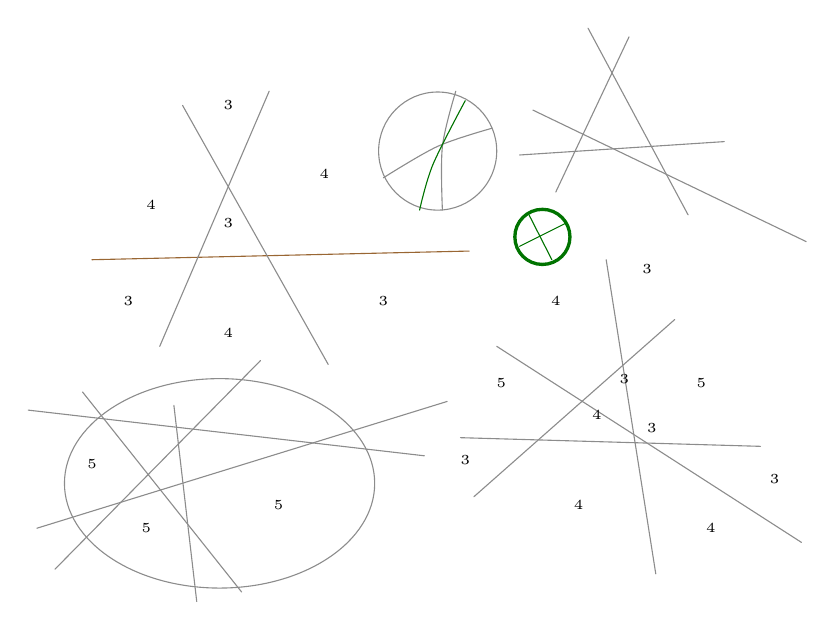
\begin{tikzpicture}[x=1mm,y=1mm,line cap=round,line join=round,font=\scriptsize]
\draw[Br] (8.7,-30.6) -- (56.6,-29.5);
\draw[pencil] (20.2,-11) -- (38.7,-43.9);
\draw[pencil] (31.2,-9.2) -- (17.3,-41.6);
\node[inner sep=1pt] at (26,-11) {\tiny $3$};
\node[inner sep=1pt] at (38.2,-19.7) {\tiny $4$};
\node[inner sep=1pt] at (16.2,-23.7) {\tiny $4$};
\node[inner sep=1pt] at (26,-26) {\tiny $3$};
\node[inner sep=1pt] at (13.3,-35.8) {\tiny $3$};
\node[inner sep=1pt] at (45.7,-35.8) {\tiny $3$};
\node[inner sep=1pt] at (26,-39.9) {\tiny $4$};
\draw[pencil] (52.6,-16.8) circle[radius=7.5];
\draw[pencil] plot[smooth, tension=0.55] coordinates {(54.9,-9.2) (53.2,-16.2) (53.2,-24.3)};
\draw[pencil] plot[smooth, tension=0.55] coordinates {(45.7,-20.2) (52.6,-16.2) (59.5,-13.9)};
\draw[Dg] plot[smooth, tension=0.55] coordinates {(50.3,-24.3) (52,-18.5) (56.1,-10.4)};
\draw[Dg,very thick] (65.9,-27.7) circle[radius=3.5];
\draw[Dg] (64.2,-24.9) -- (67.1,-30.6);
\draw[Dg] (63,-28.9) -- (68.8,-26);
\draw[pencil] (71.7,-1.2) -- (84.4,-24.9);
\draw[pencil] (76.9,-2.3) -- (67.6,-22);
\draw[pencil] (63,-17.3) -- (89,-15.6);
\draw[pencil] (64.7,-11.6) -- (99.4,-28.3);
\draw[pencil] (24.9,-59) ellipse[x radius=19.7, y radius=13.3];
\draw[pencil] (0.6,-49.7) -- (50.9,-55.5);
\draw[pencil] (1.7,-64.7) -- (53.8,-48.6);
\draw[pencil] (7.5,-47.4) -- (27.7,-72.8);
\draw[pencil] (19.1,-49.1) -- (22,-74);
\draw[pencil] (4,-69.9) -- (30.1,-43.4);
\node[inner sep=1pt] at (8.7,-56.6) {\tiny $5$};
\node[inner sep=1pt] at (15.6,-64.7) {\tiny $5$};
\node[inner sep=1pt] at (32.4,-61.8) {\tiny $5$};
\draw[pencil] (60.1,-41.6) -- (98.8,-66.5);
\draw[pencil] (57.2,-60.7) -- (82.7,-38.2);
\draw[pencil] (74,-30.6) -- (80.3,-70.5);
\draw[pencil] (55.5,-53.2) -- (93.6,-54.3);
\node[inner sep=1pt] at (79.2,-31.8) {\tiny $3$};
\node[inner sep=1pt] at (67.6,-35.8) {\tiny $4$};
\node[inner sep=1pt] at (60.7,-46.2) {\tiny $5$};
\node[inner sep=1pt] at (76.3,-45.7) {\tiny $3$};
\node[inner sep=1pt] at (72.8,-50.3) {\tiny $4$};
\node[inner sep=1pt] at (79.8,-52) {\tiny $3$};
\node[inner sep=1pt] at (86.1,-46.2) {\tiny $5$};
\node[inner sep=1pt] at (56.1,-56.1) {\tiny $3$};
\node[inner sep=1pt] at (70.5,-61.8) {\tiny $4$};
\node[inner sep=1pt] at (95.4,-58.4) {\tiny $3$};
\node[inner sep=1pt] at (87.3,-64.7) {\tiny $4$};
\end{tikzpicture}
\end{document}
